\documentclass[a4j,11pt,twoside]{jbook}
\usepackage{ascmac}
\usepackage{amsmath}
\usepackage[dvipdfmx]{graphicx}
\usepackage[dvipdfmx]{color}
\usepackage{matx}
\usepackage{manyfloat}
\usepackage{caption}
\usepackage{geometry}
\usepackage{listings,jlisting}
\usepackage{listings}
\usepackage{color}
\captionsetup{labelformat=empty,labelsep=none}
\geometry{left=25mm,right=25mm,top=28mm,bottom=25mm}

\lstset{
	language=C,
	showstringspaces=f
	basicstyle={\ttfamily\small},
	tabsize=3,
	frame=trBL,
	numbers=left,
	numberstyle={\ttfamily\small},
	breaklines=true,
	backgroundcolor={\color[gray]{.96}},
}

\begin{document}

% --- title page --- %
\title{倒立振子の安定化制御}
\author{前田 拓}
\date{2017年8月4日}
\maketitle

% --- index --- %
\pagenumbering{roman}
\tableofcontents
\listoffigures
\listoftables
\pagenumbering{arabic}

% --- main --- %

% ----- chapter 1 ----- %
% ================================= chapter 1 ================================= %
\chapter{はじめに}
\section{目的}
本実験の目的は,倒立振子系を状態空間表現を用いて安定化制御し,線形不変システムを設計することである.
具体的に,次のことを目的とする.

\begin{itemize}
    \renewcommand{\labelenumi}{(\roman{enumi})}
    \item 倒立振子が安定化制御を行っている状態において,外乱による影響で振子が傾いたとき,倒立状態に戻すことができる (不安定平衡点の安定化).
    \item 倒立振子系に一定周期のパルス入力を与え,台車を目的の変位へ移動させる.
    \item 倒立振子が入力なしで静止している状態から,台車を動かすことにより振子を振り上げ,倒立状態にする (振り上げ制御).
\end{itemize}

\section{実験装置}

\begin{figure}[htbp]
    \begin{center}
        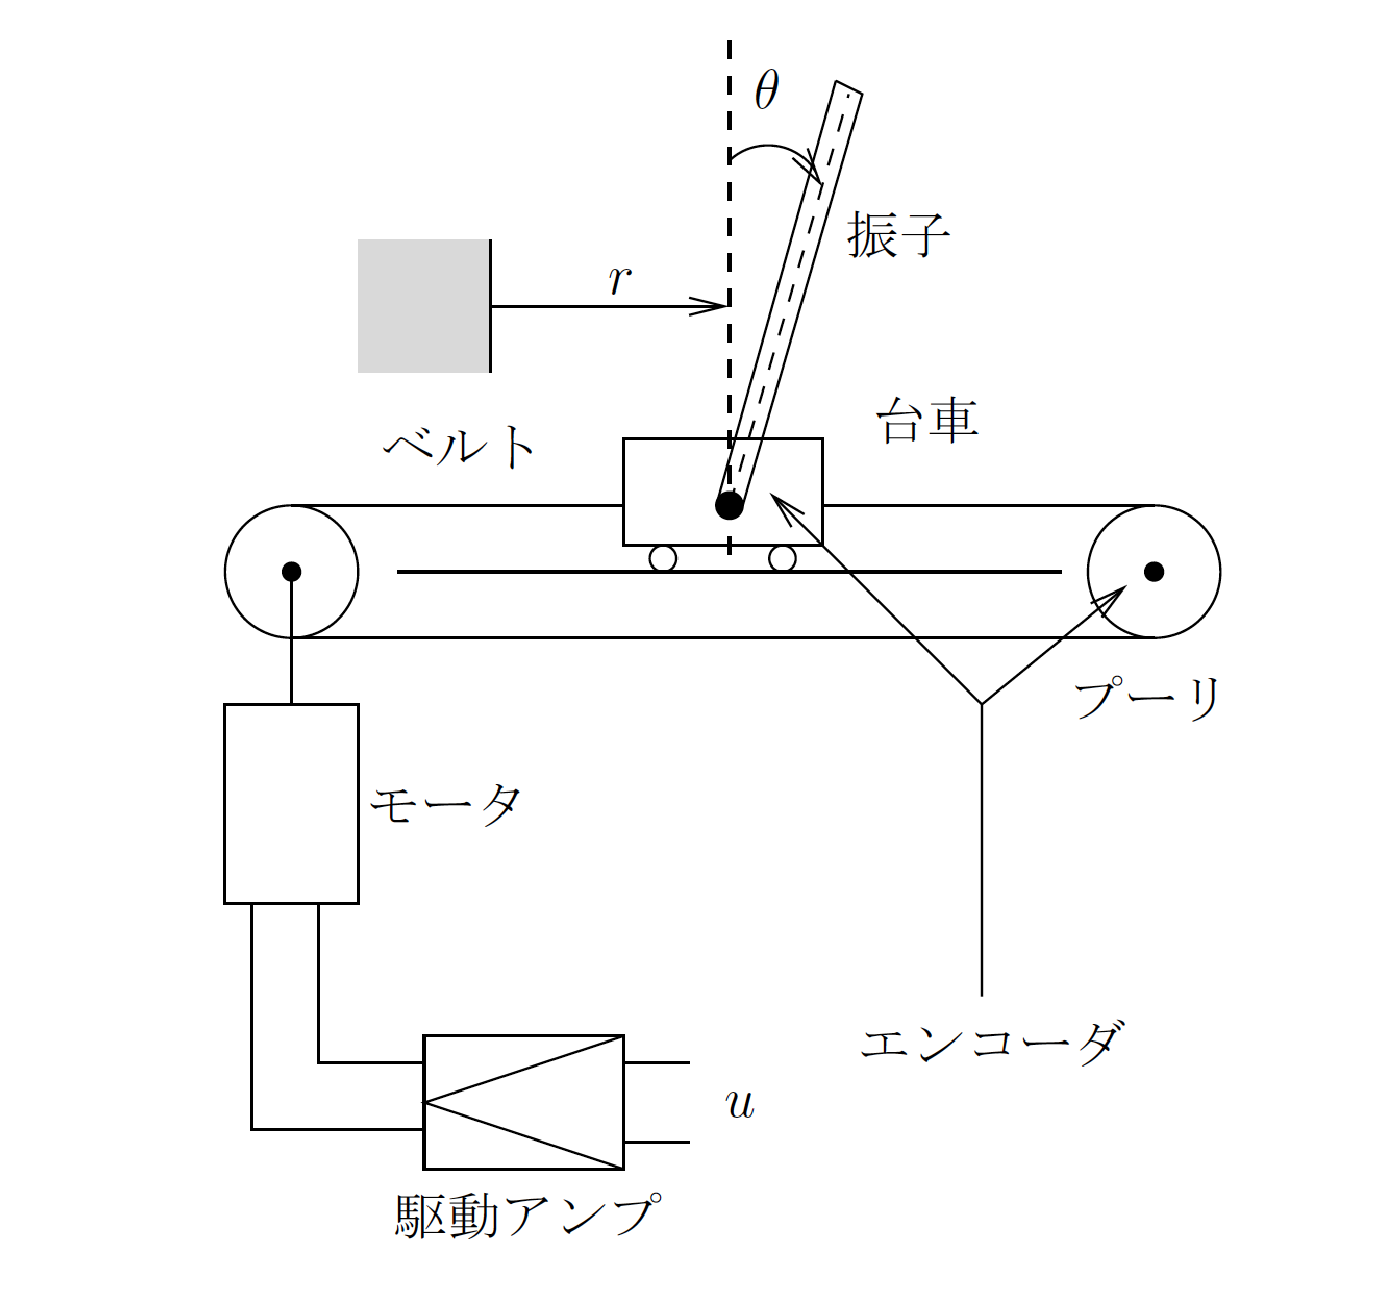
\includegraphics[width=0.6\linewidth]{model.eps}
        \caption{図\ref{pendulum}: 倒立振子系}
        \label{pendulum}
    \end{center}
\end{figure}

図\ref{pendulum}は本実験で使用する倒立振子系である.
系は,モータ,ベルト,プーリ系から成り,台車はモータからの入力によりベルト上を水平方向に動くことができる.
台車の初期状態からの変位を$r$とする.
また,鉛直方向上向きから時計回りを正の方向として,台車に取り付けられた振子が回転した角度を$\theta$とする.
ポテンショメータにより,$r$と$\theta$を測定し,入力$u$を与える.

% =============================== chapter 1 END =============================== %
% --- Chapter 1 END --- %

% ----- chapter 2 ----- %
\input{modeling.tex}
% --- Chapter 2 END --- %

% ----- chapter 3 ----- %
% ================================= chapter 3 ================================= %
\chapter{制御系設計}
\subsection{特性解析}
第\ref{chapter_modeling}章で物理パラメータの決定と数式モデルの導出を行った.
ここでは,決定したパラメータから,式(\ref{linear_k}),式(\ref{linear_general})の特性解析を行う.
倒立振子の線形モデルの状態空間表現は以下のようになる.

\begin{equation}
    A,\ B,\ Cの値
    \label{ABC}
\end{equation}

まず,行列$A$の安定判別を行う.$A$のすべての固有値に関して,実部が負であれば$A$は安定性行列である.
すなわち,$A$の固有値$\lambda_{1}$, $\lambda_{2}$, $...$に対し,

$$
    \mbox{Re}[\lambda_{i}] < 0
$$

が成立すればよい.\MaTX{}で$A$の固有値を算出した結果を表\ref{eigen_A}に示す.

\begin{table}[htbp]
    \begin{center}
        \caption{表\ref{eigen_A}: $A$の固有値}
        \begin{tabular}{|c|c|} \hline
            固有値 & Re[$\lambda_{i}$] \\ \hline \hline
            $0 + 0i$ & $0$ \\ \hline
            $-8.89 \times 10^{-2} + 6.93i$ & $-8.89 \times 10^{-2}$ \\ \hline
            $-8.89 \times 10^{-2} - 6.93i$ & $-8.89 \times 10^{-2}$ \\ \hline
            $-9.45 + 0i$ & $-9.45$ \\ \hline
        \end{tabular}
        \label{eigen_A}
    \end{center}
\end{table}

表\ref{eigen_A}から,倒立振子系のシステムは不安定である.次に,システムの可制御性,可観測性を判別する.
可制御性は,$n$をシステムの次数(倒立振子系のシステムの次数は$n = 4$)に対し,可制御性行列,

$$
    U_{C} =
    \left[
        \begin{array}{ccccc}
            B  &  AB  &  A^2B  &  \dots  &  A^{n-1}B
        \end{array}
    \right]
$$

のランクがシステムの次数と等しければ満たされる.また,可観測性行列は,

$$
    U_{o} = 
    \left[
        \begin{array}{c}
            C \\
            CA \\
            CA^2 \\
            \vdots \\
            CA^{n-1}
        \end{array}
    \right]
$$

であり,$U_{o}$のランクがシステムの次数と等しければ可観測となる.
式(\ref{ABC})において,\MaTX{}を用いて$U_{c}$, $U_{o}$のランクを計算した結果,以下のようになった.

$$
    rank[U_c] = 4,\ rank[U_o] = 4
$$

以上から,倒立振子系のシステムは不安定であり,可制御かつ可観測である.

\subsection{制御システムの構成}
図\ref{controller_system}に,倒立振子系に対する制御システムの構成を示す.

\begin{figure}[htbp]
    \begin{center}
        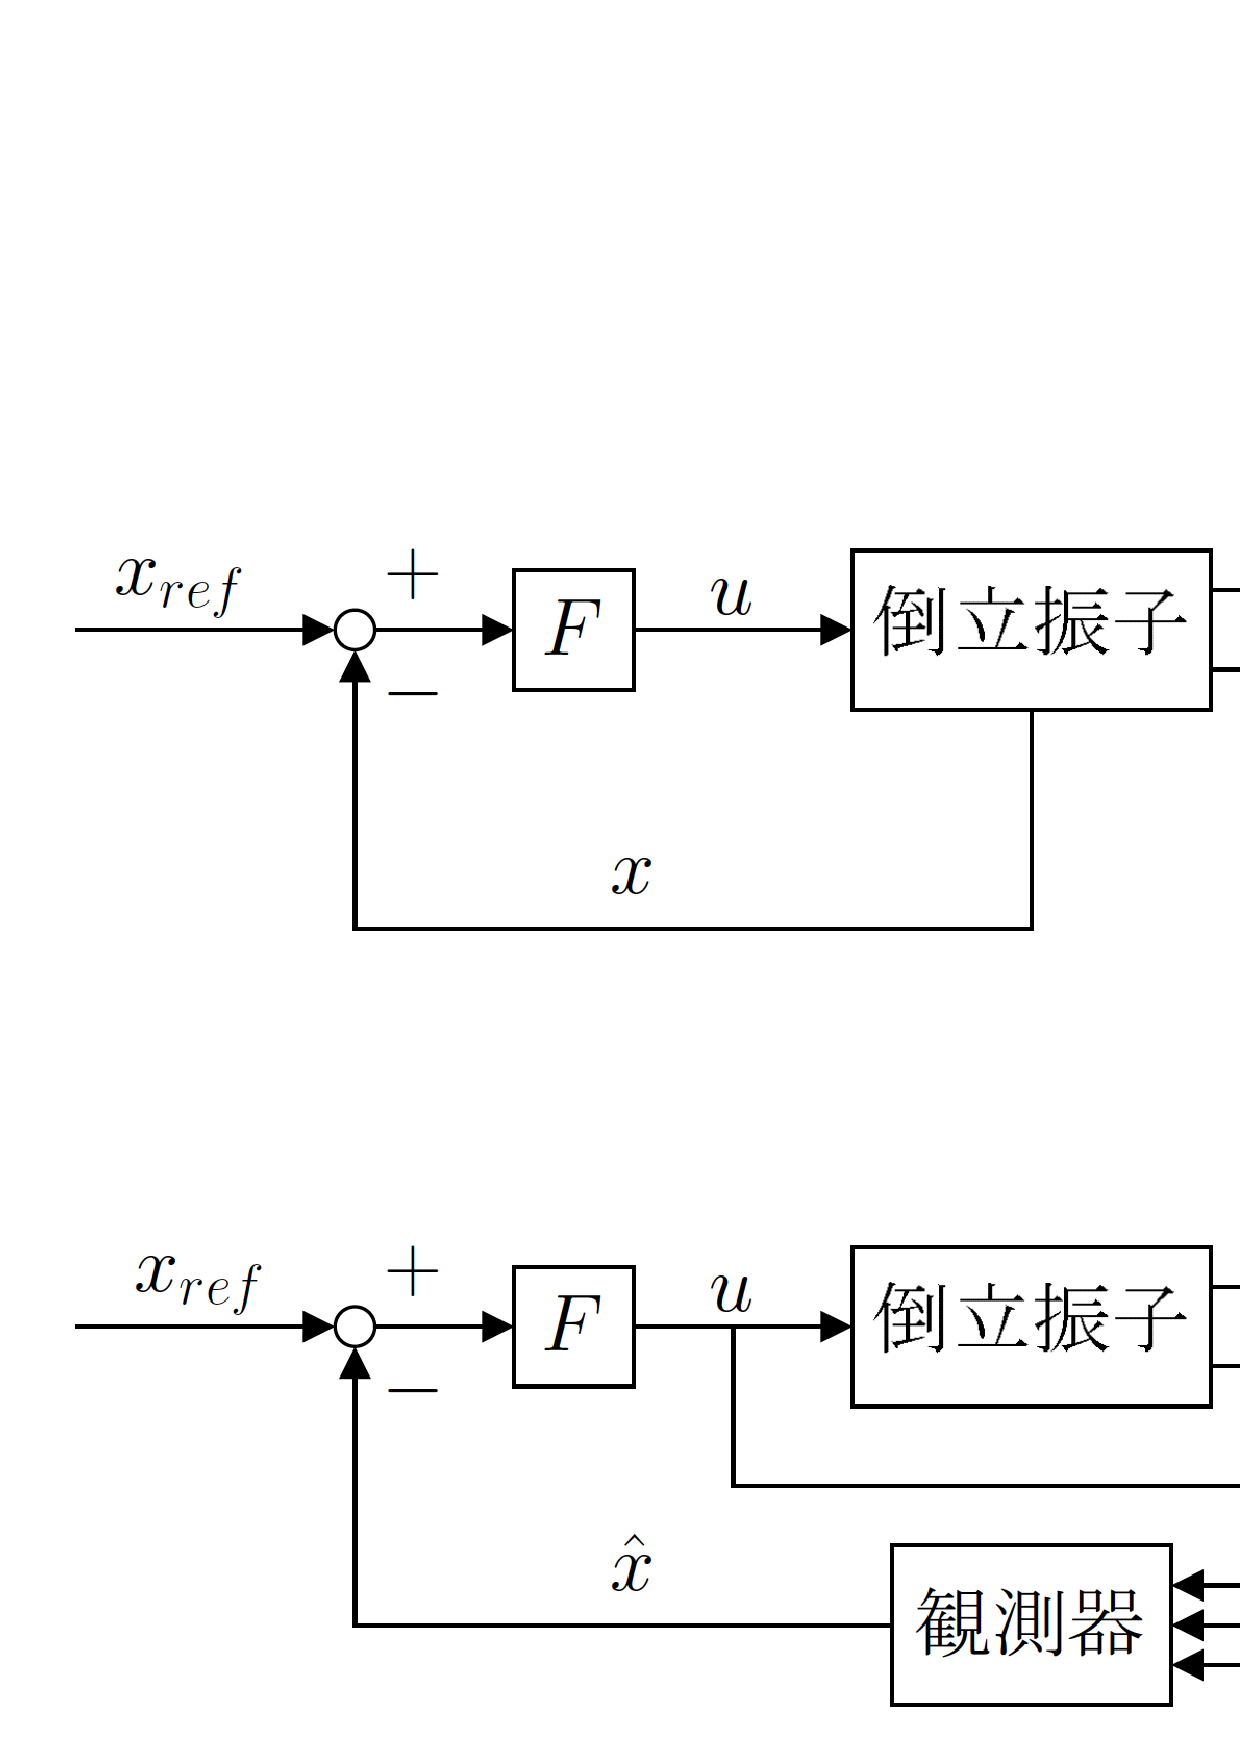
\includegraphics[width=0.6\linewidth]{controller_system.png}
        \caption{図\ref{controller_system}: 制御システムの構成}
        \label{controller_system}
    \end{center}
\end{figure}

制御系のフィードバックによる入力は,

$$
    u = -F \left( x - x_{ref} \right)
$$

ただし,

$$
    x_{ref} =
    \left[
        \begin{array}{c}
            y_{c} \\
            0 \\
            0 \\
            0
        \end{array}
    \right]
$$

であり,$y_{C}$は指定された台車位置を表す.本実験では,$\dot{r}$, $\dot{\theta}$の検出器は
用いず,状態$x$は推定値$\hat{x}$において,

\begin{equation}
    x = \lim_{t \to \infty} \hat{x}
    \label{definition_x}
\end{equation}

とする.また,式(\ref{definition_x})を満足する最小次元オブザーバ,

\begin{equation}
    \hat{z} = \hat{A}z + \hat{B}y + \hat{J}u
    \label{z_hat}
\end{equation}

\begin{equation}
    \hat{x} = \hat{C}z + \hat{D}y
    \label{x_hat}
\end{equation}

を用いる.ここで,オブザーバの次数は$2$であり,設計すべき制御システムは以下のようになる.

\begin{itemize}
    \item $F(1 \times 4)$
    \item $\hat{A}(2 \times 2)$, $\hat{B}(2 \times 2)$, 
    $\hat{J}(2 \times 1)$, $\hat{C}(4 \times 2)$, $\hat{D}(4 \times 2)$
\end{itemize}


\subsection{状態フィードバック$F$の設計}
$F$は,システムを安定化する状態フィードバック,

\begin{equation}
    u = -Fx
    \label{feedback_u}
\end{equation}

を満たすように求める.式(\ref{feedback_u})をLQ問題として解くため,$2$次形式評価関数,

\begin{equation}
    J = \int_{0}^{\infty}
    \left(
        x^{T}Qx + Ru^2
    \right)
    dt
    \label{eval2_J}
\end{equation}

\begin{equation}
    Q = \mbox{diag}(q_{1}^2, q_{2}^2, q_{3}^2, q_{4}^2), R = 1
    \label{eval2_Q}
\end{equation}

を考える.ここで,$\mbox{diag}(\dots)$は,各引数を固有値にもつ対角行列を表す.これは,

\begin{equation}
    J = \int_{0}^{\infty}
    \left(
        q_{1}^2 r^2 + q_{2}^2 \theta^2 + q_{3}^2 \dot{r}^2 + q_{4}^2 \dot{\theta}^2 + u^2
    \right)
    dt
\end{equation}

と表せるから,$q_{1}$, $q_{2}$, $q_{3}$, $q_{4}$はそれぞれ,台車位置$r$, 振子角度$\theta$,
台車速度$\dot{r}$, 振子角速度$\dot{\theta}$に対する重み係数である.
式(\ref{eval2_J}), 式(\ref{eval2_Q})を最小にする$F$は,リッカチ方程式,

$$
    A^{T}P + PA - PBR^{-1}B^{T}P + Q = 0
$$

の解$(P > 0)$に対し,

$$
    F = R^{-1}B^{T}P
$$

で与えられる.

\subsection{$\hat{A}$, $\hat{B}$, $\hat{C}$, $\hat{D}$, $\hat{J}$の設計}
式(\ref{z_hat}), 式(\ref{x_hat})が式(\ref{definition_x})を満足するための十分条件は,
ある行列$U(1 \times 4)$が存在して,

$$
    \begin{array}{c}
        UA = \hat{A}U + \hat{B}C \\
        UB = \hat{J} \\
        I = \hat{C}U + \hat{D}C
    \end{array}
$$

であり,かつ$\hat{A}$が安定性行列であることである.これらの条件を満足するオブザーバを設計するため,
Gopinathの方法を用いる.

\subsection{制御システムの離散化}
式(\ref{feedback_u}), 式(\ref{z_hat}), 式(\ref{x_hat})で示した$u,\ \hat{z},\ \hat{x}$は,
連続時間上で設計される制御器である.そこで,計算機で制御器を表現するためこれらの離散時間化を行う.
各サンプリングの間隔を$\Delta$とすると,

$$
    \begin{array}{c}
        u[k] = -F \hat{x}[k] \\
        z[k + 1] = \hat{A}_{d}z[k] + \hat{B}_{d}y[k] + \hat{J}_{d}u[k] \\
        \hat{x}[k] = \hat{C}_{d}z[k] + \hat{D}_{d}y[k]
    \end{array}
$$

と表せる.ただし,$k = 0, 1, \dots$において,

$$
    x_{ref} = 
    \left[
        \begin{array}{cc}
            \hat{A}_{d}  &  \left[
                                \begin{array}{cc}
                                    \hat{B}_{d}  &  \hat{J}_{d}
                                \end{array}
                            \right] \\
            0            &  I_{3}
        \end{array}
    \right]
    =
    \exp \Delta
    \left[
        \begin{array}{cc}
            \hat{A}  &  \left[
                            \begin{array}{cc}
                                \hat{B}  &  \hat{J}
                            \end{array}
                        \right] \\
            0        &  I_{3}
        \end{array}
    \right]
$$

である.

\subsection{振り上げ制御と安定化}
台車と振子の運動方程式は,式(\ref{del_Fh}), 式(\ref{del_Fh_Fv})から,

$$
    \begin{array}{c}
        (M + m) \ddot{r} + (ml\cos{\theta}) \ddot{\theta} 
            = au + (ml\sin{\theta}) \dot{\theta}^2 - f \dot{r} \\
        ml\cos{\theta} \ddot{r} + (J + ml^2) \ddot{\theta} 
            = mgl\sin{\theta} -c \dot{\theta}
    \end{array}
$$

で与えられる.振子が鉛直上向きのときを基準とする振子の力学的エネルギーは,

\begin{equation}
    E = \frac{1}{2} \left( J + ml^2 \right) \ddot{\theta}
        + mgl \left( \cos{\theta} - 1 \right)
\end{equation}

であり,力学的エネルギーの時間微分は,

\begin{equation}
    \frac{dE}{dt} = (J + ml) \theta \ddot{\theta}
                    - mgl \dot{\theta} \sin{\theta}
    \label{dEdt}
\end{equation}

となる.振り上げ処理を行うため,入力$u$を次のように計算する.

\begin{equation}
    u = \frac{1}{a}
        \left(
            f \dot{r} - ml \sin{\theta} \dot{\theta}^2 + ml \cos{\theta} \ddot{\theta}
            + (M + m)v
        \right)
    \label{swing_u}
\end{equation}

\begin{equation}
    v = - \frac{c \dot{\theta}}{ml\cos{\theta}} 
        + k(E - E_{0}) \mbox{sign}(\dot{\theta}\cos{\theta})
    \label{swing_v}
\end{equation}

$\mbox{sign}$は符号関数であり,引数が$0$のとき$0$を,正のとき$1$を,負のとき$-1$を返す.
式(\ref{del_Fh})に式(\ref{swing_u})を代入すると,

\begin{equation}
    \ddot{r} = v
    \label{ddot_r}
\end{equation}

を得る.式(\ref{ddot_r}), 式(\ref{swing_v})を式(\ref{del_Fh_Fv})に代入すると,

\begin{equation}
    (J + ml^2) \ddot{\theta} = mgl \sin{\theta}
                - ml \cos{\theta} (k(E - E_{0}) \mbox{sign} (\dot{\theta} \cos{\theta}))    
\end{equation}

を得る.さらに,これを式(\ref{dEdt})に代入すると,

\begin{equation*}
    \begin{split}
        \frac{dE}{dt} &= -ml \dot{\theta} \cos{\theta} (k(E - E_{0}) 
                            \mbox{sign} (\dot{\theta} \cos{\theta})) \\
                      &= -mlk(E - E_{0}) \mbox{sign} (\dot{\theta} \cos{\theta}) \dot{\theta} (\cos{\theta})
    \end{split}
\end{equation*}

となる.リアプノフ関数として,

\begin{equation}
    V = \frac{(E - E_{0})^2}{2}
\end{equation}

を考えると,$V$の時間微分,

\begin{equation}
    \begin{split}
        \frac{dV}{dt} &= (E - E_{0}) \frac{dE}{dt} \\
                      &= -mlk(E - E_{0})^2 \mbox{sign} (\dot{\theta} \cos{\theta}) \dot{\theta} (\cos{\theta}) \leq 0
    \end{split}
\end{equation}

これより,$\dot{\theta} \cos{\theta} \neq 0$のとき,$V$は減少して$0$に収束し,$E$は$E_{0}$に収束する.
実際の制御では,台車の加速度目標$v$を制限し,

$$
    u = \frac{1}{a}
        \left(
            f \dot{r} - ml \sin{\theta} \dot{\theta}^2 + ml \cos{\theta} \ddot{\theta}
            + (M + m)v
        \right)
$$

$$
    v = - \frac{c \dot{\theta}}{ml\cos{\theta}} 
        + \mbox{sat}_{ng} (k(E - E_{0}) \mbox{sign}(\dot{\theta}\cos{\theta}))
$$

とする.ただし,$\mbox{sat}_{ng}$は最小値$-ng$, 最大値$ng$の飽和関数である.また,$n$は
重力加速度と台車の加速度の比である.さらに,$k$を大きくすればより早く$E$が$E_{0}$に収束する.



% =============================== chapter 3 END =============================== %
 
% --- Chapter 3 END --- %

% ----- chapter 4 ----- %
% ================================= chapter 4 ================================= %
\chapter{シミュレーション}
目標値変更,振り上げ制御のシミュレーションを行い,重み行列,オブザーバの極,サンプリング周期,
パラメータ$k$, $n$を変更し,それぞれの変更による性能の違いを確かめる.

\subsection{重み行列変更に関するシミュレーション}
目標値変更における安定化制御で,表\ref{sim_Q}に示すパラメータを用いてシミュレーションを行う.

\begin{table}[htbp]
    \begin{center}
        \caption{表\ref{sim_Q}: 重み行列によるシミュレーションに用いるパラメータの種類}
        \begin{tabular}{|c|c|c|c|c|} \hline
            パターン & 重み行列$Q$ & オブザーバの極$P$ & サンプリング周期$dt$[s] \\ \hline \hline
            パターン1 & $Q_1$(1E6, 1E5, 1, 1) & $P_1$((-23,0), (-23,0)) & $dt_1$:0.005 \\ \hline
            パターン2 & $Q_2$(1E5, 1E6, 1, 1) & $P_2$((-23,0), (-23,0)) & $dt_2$:0.005 \\ \hline
            パターン3 & $Q_3$(1E6, 1E6, 1, 1) & $P_3$((-23,0), (-23,0)) & $dt_3$:0.005 \\ \hline
        \end{tabular}
        \label{sim_Q}
    \end{center}
\end{table}

表\ref{sim_Q}に従ってシミュレーションを行った結果を図\ref{sim_Q_r}, 図\ref{sim_Q_th}に示す.

\begin{figure}[htbp]
    \begin{minipage}{0.5\hsize}
        \begin{center}
            \includegraphics[width=1.0\linewidth]{CompareQ_r.eps}
            \caption{図\ref{sim_Q_r}: 重み行列による比較(台車位置)}
            \label{sim_Q_r}
        \end{center}
    \end{minipage}
    \begin{minipage}{0.5\hsize}
        \begin{center}
            \includegraphics[width=1.0\linewidth]{CompareQ_th.eps}
            \caption{図\ref{sim_Q_th}: 重み行列による比較(振子角度})
            \label{sim_Q_th}
        \end{center}
    \end{minipage}
\end{figure}

図\ref{sim_Q_r}から,最も重みを大きくしたパターン1をみると,たしかに台車の目標位置への収束は速くなっているが,
台車の位置を有線する一方で振子の角度の振幅は大きくなっている.一方で,振子角度の重みを最も大きくしたパターン2では,
振子角度の振幅は小さく抑えられていると同時に,台車位置の目標値への収束が3パターンの中で最も遅くなっている.

\subsection{オブザーバの極変更に関するシミュレーション}
目標値変更における安定化制御で,表\ref{sim_P}に示すパラメータを用いてシミュレーションを行う.

\begin{table}[htbp]
    \begin{center}
        \caption{表\ref{sim_P}: オブザーバの極によるシミュレーションに用いるパラメータの種類}
        \begin{tabular}{|c|c|c|c|c|} \hline
            パターン & 重み行列$Q$ & オブザーバの極$P$ & サンプリング周期$dt$[s] \\ \hline \hline
            パターン1 & $Q_1$(1E6, 1E5, 1, 1) & $P_1$((-23,0), (-23,0)) & $dt_1$:0.005 \\ \hline
            パターン2 & $Q_2$(1E6, 1E5, 1, 1) & $P_2$((-50,0), (-50,0)) & $dt_2$:0.005 \\ \hline
        \end{tabular}
        \label{sim_P}
    \end{center}
\end{table}

表\ref{sim_P}に従ってシミュレーションを行った結果を図\ref{sim_P_r}, 図\ref{sim_P_th}に示す.

\begin{figure}[htbp]
    \begin{minipage}{0.5\hsize}
        \begin{center}
            \includegraphics[width=1.0\linewidth]{CompareP_r.eps}
            \caption{図\ref{sim_P_r}: オブザーバの極による比較(台車位置)}
            \label{sim_P_r}
        \end{center}
    \end{minipage}
    \begin{minipage}{0.5\hsize}
        \begin{center}
            \includegraphics[width=1.0\linewidth]{CompareP_th.eps}
            \caption{図\ref{sim_P_th}: オブザーバの極による比較(振子角度)}
            \label{sim_P_th}
        \end{center}
    \end{minipage}
\end{figure}

台車位置,振子角度だけでは変化が表れにくいので,それぞれのオブザーバの推定誤差を用いて比較を行う.
図\ref{error_obs_r}に台車速度に関する推定誤差を,図\ref{error_obs_th}に振子角速度に関する推定誤差を示す.

\begin{figure}[htbp]
    \begin{minipage}{0.5\hsize}
        \begin{center}
            \includegraphics[width=1.0\linewidth]{error_obs_dr.eps}
            \caption{図\ref{error_obs_r}: 台車速度の推定誤差}
            \label{error_obs_r}
        \end{center}
    \end{minipage}
    \begin{minipage}{0.5\hsize}
        \begin{center}
            \includegraphics[width=1.0\linewidth]{error_obs_dth.eps}
            \caption{図\ref{error_obs_th}: 振子角速度の推定誤差}
            \label{error_obs_th}
        \end{center}
    \end{minipage}
\end{figure}

台車速度,振子角度の推定誤差ともに,オブザーバの極が負の方向に虚軸から遠いほど推定誤差が大きくなっている.
よって,このシミュレーション結果からはオブザーバの極は虚軸に近い極配置が好ましいと言える.
実際には,極の絶対値がより大きいほど推定誤差は小さくなるが,本実験で行ったシミュレーションのパラメータでは
既に極の絶対値が十分に大きく,オブザーバの極配置以外の要因により推定誤差が大きくなったと考察できる.


\subsection{サンプリング周期変更に関するシミュレーション}
目標値変更における安定化制御で,表\ref{sim_Dt}に示すパラメータを用いてシミュレーションを行う.

\begin{table}[htbp]
    \begin{center}
        \caption{表\ref{sim_Dt}: サンプリング周期によるシミュレーションに用いるパラメータの種類}
        \begin{tabular}{|c|c|c|c|c|} \hline
            パターン & 重み行列$Q$ & オブザーバの極$P$ & サンプリング周期$dt$[s] \\ \hline \hline
            パターン1 & $Q_1$(1E6, 1E5, 1, 1) & $P_1$((-23,0), (-23,0)) & $dt_1$:0.005 \\ \hline
            パターン2 & $Q_2$(1E6, 1E5, 1, 1) & $P_2$((-23,0), (-23,0)) & $dt_2$:0.01 \\ \hline
        \end{tabular}
        \label{sim_Dt}
    \end{center}
\end{table}

表\ref{sim_Dt}に従ってシミュレーションを行った結果を図\ref{sim_Dt_r}, 図\ref{sim_Dt_th}に示す.

\begin{figure}[htbp]
    \begin{minipage}{0.5\hsize}
        \begin{center}
            \includegraphics[width=1.0\linewidth]{CompareDt_r.eps}
            \caption{図\ref{sim_Dt_r}: サンプリング周期による比較(台車位置)}
            \label{sim_Dt_r}
        \end{center}
    \end{minipage}
    \begin{minipage}{0.5\hsize}
        \begin{center}
            \includegraphics[width=1.0\linewidth]{CompareDt_th.eps}
            \caption{図\ref{sim_Dt_th}: サンプリング周期による比較(振子角度)}
            \label{sim_Dt_th}
        \end{center}
    \end{minipage}
\end{figure}

オブザーバの極によるシミュレーション同様,台車位置,振子角度だけでは変化が表れにくいので,
それぞれのオブザーバの推定誤差を用いて比較を行う.
図\ref{error_dt_r}に台車速度に関する推定誤差を,図\ref{error_dt_th}に振子角速度に関する推定誤差を示す.

\begin{figure}[htbp]
    \begin{minipage}{0.5\hsize}
        \begin{center}
            \includegraphics[width=1.0\linewidth]{error_sm_dr.eps}
            \caption{図\ref{error_dt_r}: 台車速度の推定誤差}
            \label{error_dt_r}
        \end{center}
    \end{minipage}
    \begin{minipage}{0.5\hsize}
        \begin{center}
            \includegraphics[width=1.0\linewidth]{error_sm_dth.eps}
            \caption{図\ref{error_dt_th}: 振子角速度の推定誤差}
            \label{error_dt_th}
        \end{center}
    \end{minipage}
\end{figure}

図\ref{error_dt_r},図\ref{error_dt_th}から,サンプリング周期が短いほど推定誤差が小さくなっている.
サンプリング周期を大きくすると,計測するデータの間隔が大きくなってしまうため,実際の値への追従が遅れる.
よって,このシミュレーションでは意図した結果が得られたと言える.


\subsection{振り上げ制御のシミュレーション}
振り上げシミュレーションに用いたパラメータを表\ref{sim_swing}に示す.
ただし,振子が安定化制御に移行した際に用いるパラメータは表\ref{swing_stable}のパラメータを用いることとする.
また,台車位置,振子角度の制限として,台車位置はベルト中心から両方向に$0.09$[m],振子角度は
$\left[-\pi\right.,\ \left.\pi\right)$[rad]の範囲の値を取るものとする.

\begin{table}[htbp]
    \begin{center}
        \caption{表\ref{sim_swing}: 振り上げ制御のシミュレーションに用いるパラメータの種類}
        \begin{tabular}{|c|c|c|} \hline
            パターン & $k$ & $n$ \\ \hline \hline
            パターン1 & $1.0\mbox{E}3$ & $0.31$ \\ \hline
            パターン2 & $1.0\mbox{E}4$ & $0.31$ \\ \hline
            パターン3 & $1.0\mbox{E}5$ & $0.31$ \\ \hline
        \end{tabular}
        \label{sim_swing}
    \end{center}
\end{table}

\begin{table}[htbp]
    \begin{center}
        \caption{表\ref{swing_stable}: 振り上げ後の安定化制御に用いるパラメータ}
        \begin{tabular}{|c|c|c|c|} \hline
            重み行列$Q$ & オブザーバの極$P$ & サンプリング周期$dt$[s] \\ \hline \hline
            $Q$(1E6, 1E5, 1, 1) & $P$((-23,0), (-23,0)) & $dt$:0.005 \\ \hline
          \end{tabular}
        \label{swing_stable}
    \end{center}
\end{table}

表\ref{sim_swing}を用いて振り上げ制御のシミュレーションを行った結果を図\ref{sim_swing_r},
図\ref{sim_swing_th}に示す.

\begin{figure}[htbp]
    \begin{minipage}{0.5\hsize}
        \begin{center}
            \includegraphics[width=1.0\linewidth]{swing_sim_r.eps}
            \caption{図\ref{sim_swing_r}: 台車位置}
            \label{sim_swing_r}
        \end{center}
    \end{minipage}
    \begin{minipage}{0.5\hsize}
        \begin{center}
            \includegraphics[width=1.0\linewidth]{swing_sim_th.eps}
            \caption{図\ref{sim_swing_th}: 振子角度}
            \label{sim_swing_th}
        \end{center}
    \end{minipage}
\end{figure}

パラメータ$k$の値を大きくすることで,目標とする振子の運動エネルギーへの収束が速くなることが予想されたが,
本実験のシミュレーションでは$k$の値に関わらず安定化制御に移行するまでの時間に変化はなかった.
ただし,安定化制御に移行する際の台車位置はそれぞれ異なっていたため,パラメータ$k$の値によっては
台車が制限された移動範囲外にはみ出してしまう可能性がある.

% =============================== chapter 4 END =============================== %

% --- Chapter 4 END --- %

% ----- chapter 5 ----- %
% ================================= chapter 5 ================================= %
\chapter{実験}

\subsection{実験装置}

\subsection{安定化制御の実験}

\subsection{重み行列}

\subsection{オブザーバの極}

\subsection{サンプリング周期}

\subsection{振り上げ制御}

\subsection{振り上げ制御に関する考察}


% =============================== chapter 5 END =============================== % 
% --- Chapter 5 END --- %

% ----- chapter 6 ----- %
% ================================= chapter 6 ================================= %
\chapter{おわりに}
\subsection{まとめ}
今回の実験を通して、制御系のモデリングから制御器の設計、設計した制御器を用いたシミュレーション、
実験を行い、制御の一連の流れを体験することができた。また、制御器を表現するための方法として、Java,
\MaTX{}, Jamoxの3通りの手段を用い、制御系CADの特徴や、実際にプログラムを書くこととの違いを
理解することができた。シミュレーションでは意図した通りに動作するが、実験結果は異なる、あるいは逆の
挙動を示すこともあり、シミュレーションと実験は異なることを実感した。本実験を通して理解した古賀研究室の
プロダクトの特徴、制御の経験をこれからの研究に役立てたい。

\begin{thebibliography}{2}
 \bibitem{1}B.倒立振子の安定化制御,古賀雅伸
 \bibitem{2}制御工学実験第3 倒立振子の安定化制御,古賀雅伸
\end{thebibliography}

% =============================== chapter 6 END =============================== %
 
% --- Chapter 6 END --- %

% --- main END ---%
\end{document}
